% Informe final · Aprendizaje Automático I · Tasador de autos usados (Uruguay)
% Borrador generado con los números de los notebooks al 2026-11-16 (commit 1a11ecd).
% Lo marcado con \pend{...} lo tiene que completar o revisar el grupo antes de entregar.
% Límite: 6 páginas según la tabla de la consigna (la introducción dice 5): apuntar a 5.
\documentclass[11pt,a4paper]{article}

\usepackage[utf8]{inputenc}
\usepackage[T1]{fontenc}
\usepackage[spanish,es-noshorthands]{babel}
\usepackage{lmodern}
\usepackage[margin=2.2cm]{geometry}
\usepackage{graphicx}
\usepackage{booktabs}
\usepackage{xcolor}
\usepackage{amsmath}
\usepackage{caption}
\usepackage[hidelinks]{hyperref}

\graphicspath{{../notebooks/figuras/}}
\captionsetup{font=small,labelfont=bf}

% Marca de pendientes: se ve en rojo en el PDF. Buscar "\pend" antes de entregar.
\newcommand{\pend}[1]{\textcolor{red}{[PENDIENTE: #1]}}

\title{¿Está bien de precio?\\[2pt]
\large Un tasador de autos usados para Uruguay con datos de Mercado Libre}
\author{Joaquín Elías \and Federico Otero \and Nicolás Guerra \and Santiago Bruschera}
\date{Aprendizaje Automático I · Universidad de Montevideo · 23 de noviembre de 2026}

\begin{document}
\maketitle

\begin{abstract}
\noindent
Quien compra un auto usado en Uruguay no tiene una referencia pública de precio: el mismo modelo y
año se publica a precios que difieren casi al doble. Construimos un conjunto de 17.095 avisos de autos
usados de Mercado Libre Uruguay (98,5\,\% de los publicados el 28/10/2026) y ajustamos regresiones
regularizadas sobre el logaritmo del precio. Con marca, modelo, año, kilómetros, tipo de vendedor y lo
que dice el título, el modelo tasa con un error mediano de 10,1\,\% sobre avisos no vistos ($R^2 = 0{,}86$
en log), frente a 16,1\,\% de una tasación por mediana del modelo. Un auto pierde en promedio 4,4\,\% de
su precio por año a kilómetros constantes, con diferencias significativas entre marcas (de 3,2\,\% en
Suzuki a 5,1\,\% en Nissan y Mercedes-Benz). Los avisos que más se alejan del precio predicho son, en
buena parte, \pend{completar con la revisión manual de los 40 extremos}.
\end{abstract}

% ---------------------------------------------------------------------------------------------
\section{Problema y pregunta}

El 28 de octubre de 2026 había 48 Chevrolet Onix 2019 publicados en Mercado Libre
Uruguay, con precios entre USD 7.500 y USD 14.900. Una parte de esa diferencia se explica por los
kilómetros, la versión o quién vende; el resto no, y quien compra no tiene con qué compararlo.

\textbf{Pregunta principal.} ¿Qué tan bien se puede estimar el precio de un auto usado en Uruguay a
partir de los datos de su publicación, y qué publicaciones se alejan mucho del precio que predice el
modelo?

\textbf{Pregunta secundaria.} ¿Cuánto valor pierde un auto por año y por kilómetro, y cambia según la
marca?

Es un problema de aprendizaje supervisado (regresión): cada aviso trae su precio. Hay antecedentes
con datos de Mauricio \cite{pudaruth}, Alemania \cite{kihm} y Sudáfrica \cite{hendry}; con datos de
Uruguay no encontramos.

% ---------------------------------------------------------------------------------------------
\section{Datos}

\textbf{Recolección.} Escribimos un scraper propio en Python que respeta el \texttt{robots.txt} del
sitio (verificado antes de cada consulta), hace una consulta a la vez con pausas de 4 a 8\,s, no usa
la API, ni proxies, ni login, y no guarda datos personales de los vendedores. Como el sitio prohíbe
paginar, cada búsqueda se partió por marca $\times$ tipo de vendedor, luego por modelo y luego por rango
de años hasta que entrara en una página (48 avisos). Con 1.487 consultas se obtuvieron
\textbf{17.095 avisos únicos} de los 17.353 usados que informaba el sitio (\textbf{98,5\,\%}), de 105
marcas. Es una foto del mercado de un día, no una serie de tiempo.

\textbf{Variables.} Marca, modelo, versión, año, kilómetros, precio y moneda, departamento, tipo de
vendedor (particular o concesionaria) y, a partir del título, cilindrada, transmisión y combustible
cuando el título los menciona (el resto se codifica como \emph{sin dato}).

\textbf{Limpieza.} Los avisos en pesos (1,4\,\%) se pasaron a dólares con la cotización del BCU del día
\pend{reemplazar la cotización provisoria 40,255 por la oficial del 28/10 y re-correr}. Las reglas se
aplicaron en orden y cada una se registró (Cuadro~\ref{tab:limpieza}); quedaron \textbf{16.804 avisos}
de 95 marcas y 856 modelos. La regla de avisos en pesos baratos surgió del análisis de residuos
(Sección~\ref{sec:residuos}): en una primera versión, 10 de los 20 residuos más negativos eran avisos en
pesos, la mayoría cuotas o entregas iniciales.

\begin{table}[h]
\centering\small
\begin{tabular}{lrr}
\toprule
Regla & Sacadas & Quedan \\
\midrule
Avisos obtenidos                                        &     &17.095 \\
0\,km (km $\le 1$ y año $\ge 2025$)                     & 49 & 17.046 \\
Km sin informar (km $\le 1$ y año $< 2025$)             & 45 & 17.001 \\
Km de relleno ($> 1.000.000$, ej.\ 9.999.999)           & 72 & 16.929 \\
Precio $>$ USD 150.000                                  & 36 & 16.893 \\
En pesos y $<$ USD 3.000 (cuota o moneda mal cargada)   & 86 & 16.807 \\
Avisos de compra (``Compro autos'')                     &  3 & 16.804 \\
\bottomrule
\end{tabular}
\caption{Reglas de limpieza, en el orden en que se aplicaron.}
\label{tab:limpieza}
\end{table}

\textbf{Avisos repetidos.} Hay 406 avisos que comparten marca, modelo, año, kilómetros y precio con
otro: con alta probabilidad, el mismo auto publicado dos o tres veces. Si un gemelo cae en
entrenamiento y otro en test, el modelo ``ya vio'' la respuesta y el error de test sale optimista. Por
eso cada grupo de gemelos va entero a un solo lado, tanto en la partición train/test como en la
validación cruzada.

% ---------------------------------------------------------------------------------------------
\section{Método}

\textbf{Variable objetivo.} El precio tiene cola larga a la derecha (asimetría 3,46); su logaritmo es
casi simétrico (0,51). Además, en log los errores son relativos (equivocarse en USD 2.000 no es lo
mismo en un auto de 5.000 que en uno de 50.000) y los coeficientes se leen como variaciones porcentuales:
\[
\log(\text{precio}) = \beta_0 + \beta_1\,\text{antigüedad} + \beta_2 \log(\text{km})
+ \text{marca} + \text{modelo} + \text{vendedor} + \text{indicios del título} + \varepsilon .
\]

\textbf{Partición.} 80\,\% entrenamiento (13.450 avisos) y 20\,\% test (3.354), agrupando por gemelos
(\texttt{GroupShuffleSplit}). Test se usó una sola vez, al final.

\textbf{Modelos.}
(1) \emph{Base}: la mediana del log-precio del modelo en entrenamiento (la de la marca si el modelo no
aparece). Es la tasación de sentido común; si la regresión no le gana, no aporta.
(2) \emph{Ridge} y (3) \emph{Lasso} con variables categóricas en \emph{one-hot} y numéricas
estandarizadas.

\textbf{Hiperparámetros} por validación cruzada de 5 particiones agrupadas (\texttt{GroupKFold}) dentro
de entrenamiento: la regularización $\alpha$; un \emph{umbral} de avisos por debajo del cual un modelo
de auto pasa a la categoría ``otro de la marca'' (1, 2, 3, 5, 10 o 20; los conteos se calculan en cada
partición de entrenamiento para no filtrar información); y si cada marca tiene su propia pendiente de
depreciación (interacción antigüedad $\times$ marca).

% ---------------------------------------------------------------------------------------------
\section{Resultados}

\subsection{¿Qué tan bien se estima el precio?}

\begin{table}[h]
\centering\small
\begin{tabular}{lccccc}
\toprule
Modelo & RMSE (log) & $R^2$ (log) & MAE (USD) & RMSE (USD) & Error mediano \\
\midrule
Base: mediana por modelo & 0,343 & 0,670 & 4.236 & 8.254 & 16,1\,\% \\
\textbf{Ridge}           & \textbf{0,220} & \textbf{0,863} & \textbf{2.665} & \textbf{5.811} & \textbf{10,1\,\%} \\
Lasso                    & 0,226 & 0,856 & 2.750 & 5.948 & 10,3\,\% \\
\bottomrule
\end{tabular}
\caption{Desempeño en test (3.354 avisos no vistos). Error mediano: mediana de
$|\text{predicho}/\text{real} - 1|$.}
\label{tab:resultados}
\end{table}

Ridge reduce el error mediano de 16,1\,\% a 10,1\,\% respecto de la base (Cuadro~\ref{tab:resultados}).
Lasso no mejora a Ridge: con 856 modelos, casi todas las variables aportan algo y no hay ganancia en
anular coeficientes. El mejor umbral fue 1, es decir, \emph{no} agrupar modelos raros: el RMSE de
validación sube de 0,234 (umbral 1) a 0,276 (umbral 20). La regularización de Ridge ya achica los
coeficientes de modelos con pocos avisos, y agruparlos tira información útil. La interacción
antigüedad $\times$ marca para todas las marcas empeora la validación (0,240 contra 0,234): le da una
pendiente propia a marcas con uno o dos avisos.

El error no es parejo: es menor en el centro de la distribución (8--9\,\% de error mediano entre los
deciles 4 y 7 de precio predicho) y mayor en los extremos (12\,\% en el decil más barato, 15,5\,\% en el
más caro), donde hay menos avisos y más variedad de versiones.

\subsection{Avisos fuera de mercado}
\label{sec:residuos}

Definimos el residuo como $\log(\text{precio publicado}) - \log(\text{precio predicho})$; un residuo de
$+0{,}2$ es un aviso $\approx$22\,\% más caro de lo que predice el modelo. Sobre test, la mitad de los avisos
está a menos de $\pm$10,2\,\% de lo predicho, y no hay sesgo global (mediana del residuo 0,000).
Consideramos \emph{fuera de mercado} al 10\,\% más alejado: por debajo de $-27$\,\% o por encima de
$+36$\,\% (percentiles 5 y 95; Figura~\ref{fig:residuos}).

\begin{figure}[h]
\centering
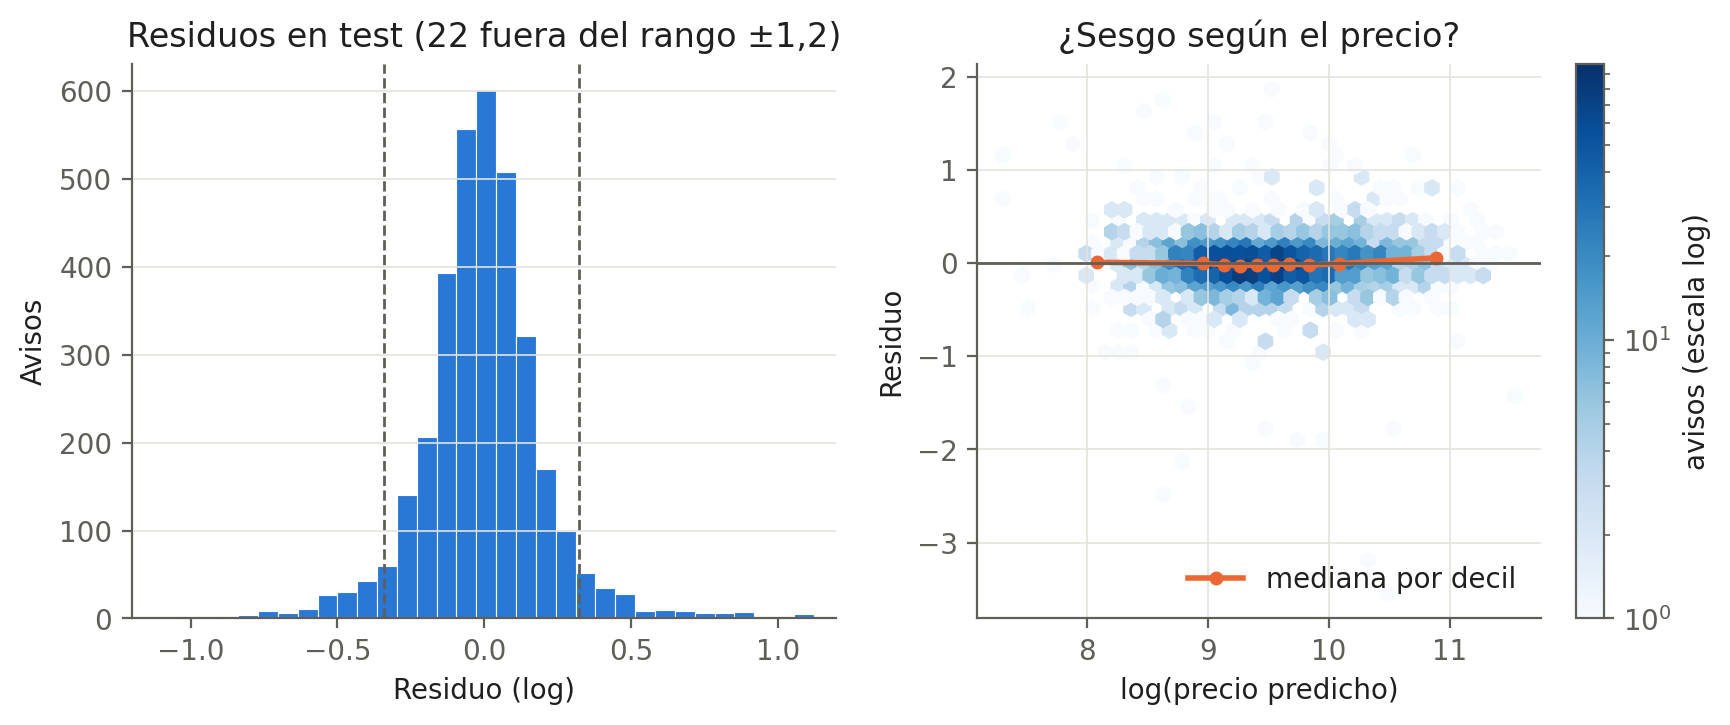
\includegraphics[width=\linewidth]{04_residuos.png}
\caption{Residuos en test. Izquierda: distribución, con los percentiles 5 y 95. Derecha: residuo
contra precio predicho; la mediana por decil se mantiene cerca de cero.}
\label{fig:residuos}
\end{figure}

Revisamos a mano los 20 avisos más por debajo y los 20 más por encima:
\pend{completar con data/extremos\_revisar.csv. Contar cuántos son error de carga (precio o año mal
puestos: p.\,ej.\ Daihatsu Cuore ``2027'' con 240.000\,km), versiones que el modelo no distingue
(AMG, M540i, Corolla GR, motorhome), estado del auto, u oportunidades/caros sin explicación aparente}.
\pend{Una o dos frases de conclusión: ¿el residuo sirve más para detectar errores de carga o para
detectar oportunidades?}

\subsection{Depreciación}

Leyendo los coeficientes de Ridge (en unidades originales), a marca, modelo y kilómetros constantes:

\begin{itemize}
\item un auto pierde \textbf{4,4\,\% de su precio por año};
\item duplicar los kilómetros le resta \textbf{4,4\,\%} (elasticidad $-0{,}065$). El efecto es chico porque
kilómetros y antigüedad están correlacionados (0,45): la antigüedad ya captura la mayor parte;
\item por el mismo auto, una concesionaria pide \textbf{2,8\,\% más} que un particular.
\end{itemize}

Para la pregunta por marca, reajustamos dando pendiente propia solo a las 13 marcas con al menos 300
avisos en entrenamiento; el resto comparte una pendiente común. Los intervalos de confianza del 95\,\% se
obtuvieron por \emph{bootstrap} de grupos de gemelos (200 repeticiones). Las diferencias son reales:
Suzuki pierde 3,2\,\% por año (IC 2,9--3,6) y Nissan 5,1\,\% (4,7--5,5), con intervalos que no se solapan
(Figura~\ref{fig:marcas}). Pero casi no mejoran la predicción: el RMSE de validación pasa de 0,2340 a
0,2332, muy por debajo de la variación entre particiones (0,013).

\begin{figure}[h]
\centering
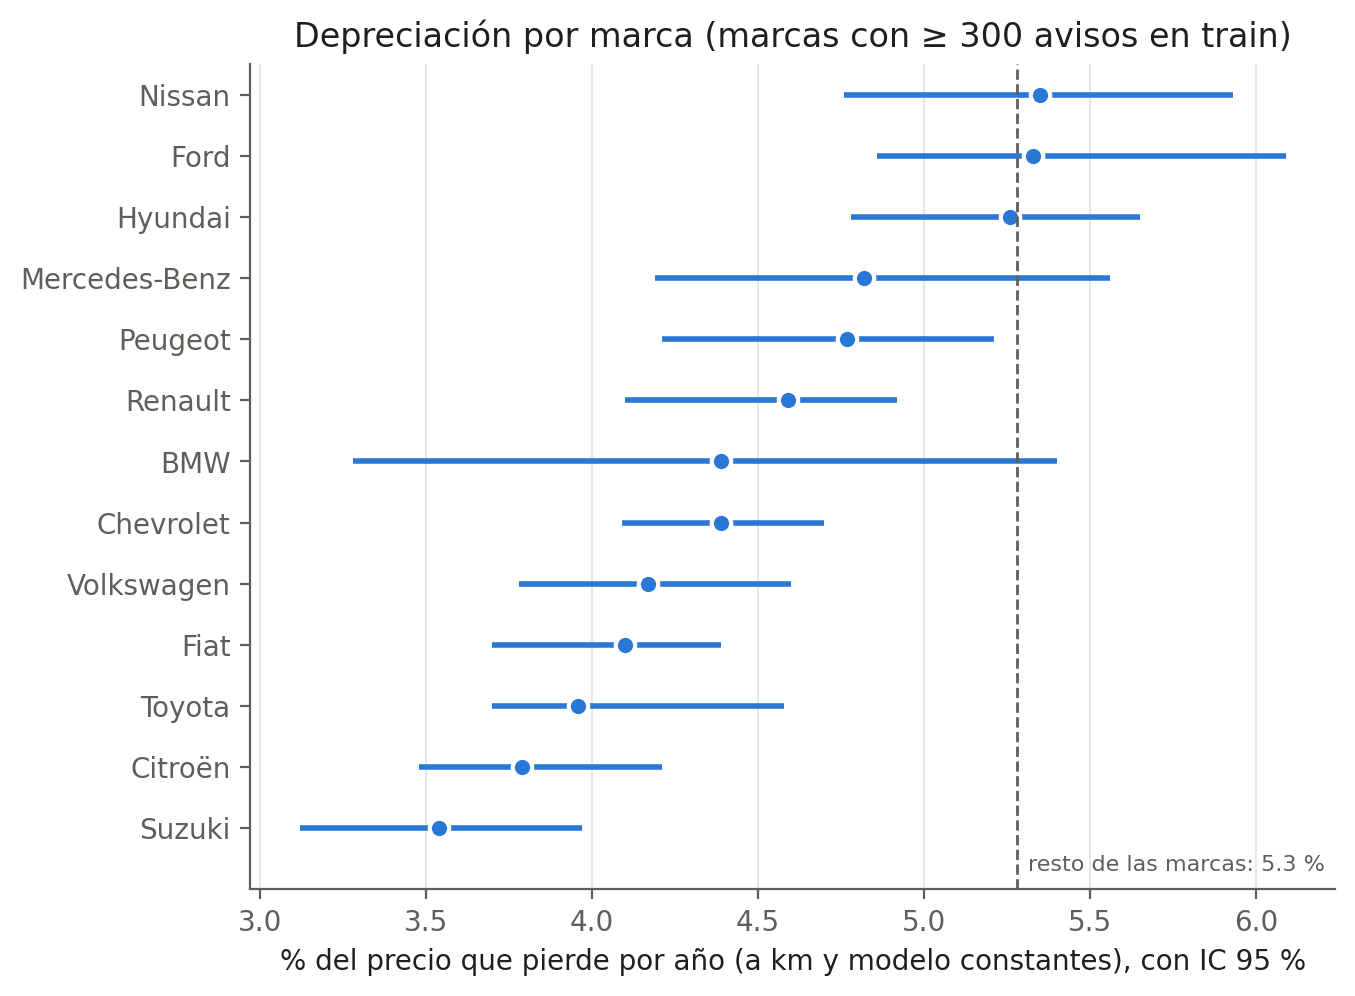
\includegraphics[width=0.78\linewidth]{05_depreciacion_marca_ic.png}
\caption{Porcentaje del precio que se pierde por año, por marca, con intervalo de confianza del 95\,\%.
La línea punteada es la pendiente común del resto de las marcas.}
\label{fig:marcas}
\end{figure}

Estas pendientes son menores que las que surgen de comparar medianas por antigüedad (6,5\,\% por año en
Chevrolet, 7,3\,\% en Nissan): sin controlar por kilómetros y modelo, a la antigüedad se le atribuye
también que los autos viejos tienen más kilómetros y son de modelos más baratos.

% ---------------------------------------------------------------------------------------------
\section{Limitaciones}

\begin{itemize}
\item \textbf{Precio publicado, no precio de venta.} El modelo aprende lo que se pide, no lo que se paga.
\item \textbf{El modelo no ve el estado del auto} (choques, mantenimiento) ni la versión exacta más allá
de lo que dice el título: es la principal fuente de residuos grandes.
\item \textbf{Muestra no aleatoria en búsquedas grandes.} Cuando una búsqueda tenía más de 48 avisos, el
sitio elegía cuáles mostrar. Pasó en dos casos (Chevrolet Montana 2024 y Onix 2023 de concesionaria).
\item \textbf{Una sola fecha.} No se puede decir nada sobre cómo cambian los precios en el tiempo.
\item \textbf{Cotización.} \pend{si sigue siendo la provisoria, decirlo acá}.
\end{itemize}

% ---------------------------------------------------------------------------------------------
\section{Conclusiones}

\pend{Tres o cuatro frases: respuesta a la pregunta principal (10\,\% de error típico, 6 puntos mejor que
la mediana del modelo), qué son los avisos fuera de mercado según la revisión manual, y la respuesta a la
secundaria (4,4\,\% por año, diferencias reales entre marcas que no cambian la tasación). Posible
aplicación: una herramienta que marque avisos a revisar.}

\medskip
\noindent\textbf{Reproducibilidad.} Código, datos y notebooks en
\url{https://github.com/JBEC2006/tasador-autos-uy} \pend{confirmar acceso del docente}. Los tres
notebooks (\texttt{01\_limpieza\_eda}, \texttt{02\_modelos}, \texttt{03\_residuos\_depreciacion})
corren de punta a punta en menos de dos minutos.

\begin{thebibliography}{9}
\small
\bibitem{pudaruth} S.~Pudaruth (2014). \pend{título, revista, volumen y páginas: ver diapositiva 10
de la propuesta y la fuente original}. Datos de Mauricio.
\bibitem{kihm} A.~Kihm y C.~Vance (2016). \pend{título, revista, volumen y páginas}. Datos de Alemania.
\bibitem{hendry} Hendry y Priilaid (2025). \pend{nombres, título, revista}. Datos de Sudáfrica.
\end{thebibliography}

\end{document}
